\documentclass{snamc2013}

%%%%%%%%%%%%%%%%%%%%%%%%%%%%%%%%%%%%%%%%%%%%%%%%%%%%%%%%%%%%%%%%%%%%%%%%%%%%%%%%
\usepackage{graphicx}  % allows inclusion of graphics
\usepackage{booktabs}  % nice rules (thick lines) for tables
\usepackage{microtype} % improves typography for PDF
\usepackage{tabls}
\usepackage{afterpage}
\usepackage{amssymb}
\usepackage{amsfonts}
\usepackage{amsmath}
\usepackage[mathcal]{euscript}
\usepackage{tmath}
\usepackage[section]{placeins}

\usepackage[breaklinks=true,colorlinks=true,linkcolor=black,citecolor=black]{hyperref}

%%%%%%%%%%%%%%%%%%%%%%%%%%%%%%%%%%%%%%%%%%%%%%%%%%%%%%%%%%%%%%%%%%%%%%%%%%%%%%%%
\title{A Multiple-Set Overlapping-Domain Decomposed Monte Carlo
  Synthetic Acceleration Method for Linear Systems}

\author[1]{Stuart R. Slattery}
\author[2]{Thomas M. Evans}
\author[1]{Paul P.H. Wilson}

\affil[1]{University of Wisconsin - Madison, Engineering Physics
  Department, 1500 Engineering Dr., Madison, WI 53706}
\affil[2]{Oak Ridge National Laboratory, Reactor and Nuclear Systems
  Division, 1 Bethel Valley Rd., Oak Ridge, TN 37831}

\abstract{We present a multiple-set overlapping-domain decomposed
  strategy for parallelizing the Monte Carlo Synthetic Acceleration
  method. Monte Carlo Synthetic Acceleration methods use the
  Neumann-Ulam class of Monte Carlo solvers for linear systems to
  accelerate a fixed-point iteration sequence. Effective parallel
  algorithms for these methods require the parallelization of the
  underlying Neumann-Ulam solvers. To do this in a domain decomposed
  environment, we borrow strategies traditionally implemented in Monte
  Carlo particle transport to parallelize the problem. The parallel
  Neumann-Ulam and multiple-set overlapping-domain decomposition
  algorithm is presented along with parallel scaling data for the
  resulting implementation using the Titan Cray XK7 machine at Oak
  Ridge National Laboratory.}

\keywords{MCSA, Monte Carlo, domain decomposition, linear solvers,
  parallel computing}

\begin{document}
%%%%%%%%%%%%%%%%%%%%%%%%%%%%%%%%%%%%%%%%%%%%%%%%%%%%%%%%%%%%%%%%%%%%%%%%%%%%%%%%
\section{Introduction}

For some time, the particle transport community has utilized Monte
Carlo methods for the solution of transport problems
\cite{lewis_computational_1993}. The partial differential equation
(PDE) community has focused on various deterministic methods for
solutions to linear problems \cite{saad_iterative_2003,
  kelley_iterative_1995}. In between these two areas are a not widely
known group of Monte Carlo methods for solving sparse linear systems
\cite{forsythe_matrix_1950, hammersley_monte_1964,
  halton_sequential_1962, halton_sequential_1994}. In recent years,
these methods have been further developed for radiation transport
problems in the form of Monte Carlo Synthetic Acceleration (MCSA)
\cite{evans_monte_2009, evans_monte_2012} but have yet to be applied
to more general sparse linear systems commonly generated by the
computational physics community. Compared to other methods in this
regime, MCSA offers three attractive qualities; (1) the physics
operator need not be symmetric or positive-definite, (2) the
stochastic nature of the solution method potentially provides a
natural solution to some aspects of the issue of resiliency, and (3)
is amenable to parallelization using modern methods developed by the
transport community \cite{wagner_hybrid_2010}. The development of a
parallel MCSA algorithm using these techniques is the primary
contribution of this work.

As leadership class machines move beyond the petascale, new algorithms
must be developed that leverage their strengths and adapt to their
shortcomings. Basic research is required now to advance methods in
time for these new machines to become operational. As machines begin
to operate at hundreds of petaflops peak performance and beyond,
trends toward reduced energy consumption will require incredibly high
levels of concurrency to achieve the desired computation rates
\cite{kogge_using_2011}. The end result of these hardware changes is
that the larger number of low-powered processors will be prone to both
soft failures such as bit errors in floating point operations and hard
failures where data cannot be recovered. Because these failures are
predicted to be common, resilient solver technologies are required to
overcome these events at the application level. With linear solvers
based on Monte Carlo techniques, such issues are potentially
alleviated by statistical arguments. In the case of soft failures,
isolated floating point errors in the Monte Carlo simulation are
absorbed within tally statistics. Completely losing memory during a
hard failure is treated as a high variance event where some portion of
the Monte Carlo histories and subsequently the solution are lost with
other histories maintained by replicating the problem and combining
the results through superposition.

In this paper, we will present the Monte Carlo methods of Neumann and
Ulam and then outline Monte Carlo Synthetic Acceleration methods. We
then present a parallel algorithm for MCSA based on the work of
Brunner and Brantley \cite{brunner_efficient_2009} and Wagner
et. al. \cite{wagner_hybrid_2010}. Using this algorithm, we perform a
series of scaling studies to characterize parallel
performance. Finally, we summarize the results and offer future work
that may improve the algorithm.

%%%%%%%%%%%%%%%%%%%%%%%%%%%%%%%%%%%%%%%%%%%%%%%%%%%%%%%%%%%%%%%%%%%%%%%%%%%%%%%%
\section{Monte Carlo Methods}
Monte Carlo Synthetic Acceleration methods rely on the Neumann-Ulam
class of linear solvers to accelerate a stationary method. These Monte
Carlo methods work by sampling a distribution with an expectation
value equivalent to that of the inverted operator. Neumann and Ulam's
work on these solvers was first published in 1950 by Forsythe and
Leibler \cite{forsythe_matrix_1950}. In the following decade, the
books of Hammersley and Handscomb \cite{hammersley_monte_1964} and
Spanier and Gelbard \cite{spanier_monte_1969} present additional
detail on the methods. In this section we briefly present the
Neumann-Ulam Monte Carlo method for solving linear systems and then
present Monte Carlo Synthetic Acceleration. We refer the reader to
\cite{evans_monte_2009} and \cite{evans_monte_2012} for a more
detailed explanation and analysis of MCSA and the Neumann-Ulam
methods.

\subsection{Neumann-Ulam Method}
We seek solutions of the general linear problem in the following form:
\begin{equation}
  \mathbf{A} \mathbf{x} = \mathbf{b}\:,
  \label{eq:linear_problem}
\end{equation}
where $\mathbf{A} \in \mathbb{R}^{N \times N}$ is a matrix operator
such that $\mathbf{A} : \mathbb{R}^{N} \rightarrow \mathbb{R}^{N}$,
$\mathbf{x} \in \mathbb{R}^N$ is the solution vector, and $\mathbf{b}
\in \mathbb{R}^N$ is the forcing term.  For a given linear operator
$\mathbf{A}$, we can use diagonal splitting to define the
\textit{iteration matrix}, $\mathbf{H}$:
\begin{equation}
  \mathbf{H} = \mathbf{I} - \mathbf{A}\:,
  \label{eq:linear_mc_iteration_matrix}
\end{equation}
such that we are solving the system:
\begin{equation}
  \mathbf{x} = \mathbf{H} \mathbf{x} + \mathbf{b}\:.
  \label{eq:richardson_split}
\end{equation}
We can then form an alternative representation for $\mathbf{A}^{-1}$
by generating the \textit{Neumann series} solution:
\begin{equation}
  \mathbf{A}^{-1}\mathbf{b} = \sum_{k=0}^{\infty}
  \mathbf{H}^k\mathbf{b} = \mathbf{x}\:,
  \label{eq:neumann_solution}
\end{equation}
which will converge if the spectral radius of $\mathbf{H}$ is less
than 1. If we expand the summation with a succession of matrix-vector
multiply operations, we arrive at an alternative perspective of this
summation by considering the $i^{th}$ component of the solution
vector:
\begin{equation}
  x_i = \sum_{k=0}^{\infty}\sum_{i_1}^{N}\sum_{i_2}^{N}\ldots
  \sum_{i_k}^{N}h_{i,i_1}h_{i_1,i_2}\ldots h_{i_{k-1},i_k}b_{i_k}\:,
  \label{eq:expanded_neumann_solution}
\end{equation}
which can interpreted as a series of transitions between states,
\begin{equation}
 \nu = i \rightarrow i_1 \rightarrow \cdots \rightarrow i_{k-1}
 \rightarrow i_{k}\:,
  \label{eq:mc_walk_permutation}
\end{equation}
in $\mathbf{H}$ where $\nu$ is interpreted as a particular sequence
permutation. We can generate these sequences of transitions through
Monte Carlo random walks by assigning them both a probability and
weight. Using the adjoint form \cite{spanier_monte_1969},
probabilities are column-scaled:
\begin{equation}
  p_{ij} = \frac{|h_{ji}|}{\sum_j |h_{ji}|}\:,
  \label{eq:adjoint_probability}
\end{equation}
such that we expect to select a new state, $j$, from the current state
in the random walk, $i$, by sampling the probability distribution
function formed by the $i^{th}$ row of the probability matrix. The
transition weight is then defined as:
\begin{equation}
  w_{ij} = \frac{h_{ji}}{p_{ij}}\:.
  \label{eq:adjoint_weight}
\end{equation}
The initial state $i_0$ of the random walk is determined by sampling
the source vector $\mathbf{b}$ with initial probabilities and weights:
\begin{equation}
  P_{(i_0=i)}(\nu) = \frac{|b_i|}{||\mathbf{b}||_1},\ \ \ W_0 =
  ||\mathbf{b}||_1 \frac{b_i}{|b_i|}\:.
  \label{eq:adjoint_starting_params}
\end{equation}
The contribution to the solution in state $j$ from a particular random
walk permutation of $k$ events is then the \textit{collision
  estimator}:
\begin{equation}
  X_{j}(\nu) = \sum_{m=0}^k W_{m} \delta_{i_m,j}\:,
  \label{eq:adjoint_permutation_contribution}
\end{equation}
where the Kronecker delta indicates that the tally contributes only in
the current state, $i_m$, of the random walk and 
\begin{equation}
  W_{m} = W_0 w_{i_0,i_1} w_{i_1,i_2} \cdots w_{i_{m-1},i_m}\:.
  \label{eq:adjoint_permutation_weight}
\end{equation}
Finally, the expectation value using all permutations is:
\begin{equation}
  E\{X_j\} = \sum_{\nu} P_{\nu} X_{j}(\nu)\:,
  \label{eq:adjoint_expectation_value}
\end{equation}
with
\begin{equation}
  P_{\nu} = P_{(i_0=i)} p_{i,i_1} p_{i_1,i_2} \cdots p_{i_{k-1},i_k}\:.
  \label{eq:adjoint_permutation_probability}
\end{equation}
Finally, we set a criteria for random walk termination by setting a
\textit{relative weight cutoff}:
\begin{equation}
  W_f = W_c W_0\:,
  \label{eq:relative_weight_cutoff}
\end{equation}
where $W_c$ is a user-defined cutoff value. The random walk will then
be terminated after $m$ steps if $W_m < W_f$.

\subsection{Monte Carlo Synthetic Acceleration}
Using the ideas of Halton's residual method
\cite{halton_sequential_1994}, Evans and Mosher recently developed a
Monte Carlo solution method that was not prohibited severely by the
quality of the initial guess for the system \cite{evans_monte_2009}
and later applied it more rigorously as a solution mechanism for the
radiation diffusion equation \cite{evans_monte_2012}. With their new
methods, they achieved identical numerical results when compared to
conventional subspace methods and observed better performance with
respect to time to solution. Their approach was instead to use
residual Monte Carlo as a synthetic acceleration for a stationary
method.

The \textit{Fixed-Point Monte Carlo Synthetic Acceleration} method is
defined as:
\begin{subequations}
  \begin{gather}
    \label{eq:mcsa_1}
    \mathbf{r}^{k} = \mathbf{b} - \mathbf{A}\mathbf{x}^{k}\:,\\
    \label{eq:mcsa_2}
    \mathbf{x}^{k+1/2} = \mathbf{x}^k + \mathbf{r}^k\:,\\
    \label{eq:mcsa_3}
    \mathbf{r}^{k+1/2} = \mathbf{b} - \mathbf{A}\mathbf{x}^{k+1/2}\:,\\
    \label{eq:mcsa_4}
    \mathbf{A}\delta\mathbf{x}^{k+1/2} = \mathbf{r}^{k+1/2}\:,\\
    \label{eq:mcsa_5}
    \mathbf{x}^{k+1} = \mathbf{x}^{k+1/2} + \delta \mathbf{x}^{k+1/2}\:,
  \end{gather}
  \label{eq:mcsa}
\end{subequations}
where $\mathbf{r}$ is the residual vector, $\delta\mathbf{x}$ is the
Monte Carlo correction vector, and $k$ indicates the iteration
index. Here, a Neumann-Ulam Monte Carlo method is used to generate the
solution correction in Eq~(\ref{eq:mcsa_4}) using the residual as
source and Richardson's iteration in Eq~(\ref{eq:mcsa_2}) has been
rewritten as a residual correction. Using Monte Carlo in this way
achieves the same effect as Halton's method, decoupling its
convergence rate from the overall convergence rate of the method. For
the Neumann-Ulam method, a set number of random walk permutations is
specified to generate the correction at each MCSA iteration. Adding
more histories to the Neumann-Ulam sequence reduces the statistical
uncertainty in $\delta\mathbf{x}$ and further accelerates the
fixed-point iteration. In addition to the Monte Carlo solver
parameters dictating the number of histories and weight cutoff, the
outer MCSA iterations also have the following stopping criteria:
\begin{equation}
  ||\mathbf{r}||_\infty < \epsilon \ ||\mathbf{b}||_\infty\:,
  \label{eq:mcsa_stopping_criteria}
\end{equation}
where $\epsilon$ is a user-defined tolerance.

%%%%%%%%%%%%%%%%%%%%%%%%%%%%%%%%%%%%%%%%%%%%%%%%%%%%%%%%%%%%%%%%%%%%%%%%%%%%%%%%
\section{Parallel Algorithms}
In this section we devise a parallel algorithm for the Neumann-Ulam
Monte Carlo method based on the multiple-set overlapping-domain
decomposition algorithm and a parallel algorithm for the MCSA
iteration that leverages the parallel Monte Carlo algorithm and
general parallel matrix-vector operations.

\subsection{Parallel Neumann-Ulam Algorithm}
In the literature, current implementations of parallel Neumann-Ulam
methods have been limited to full domain replication with parallelism
exploited through individual histories
\cite{alexandrov_efficient_1998}. For high performance computing
environments, domain decomposition strategies have been identified as
important for Monte Carlo applications
\cite{brunner_comparison_2006,siegel_analysis_2012}. In a domain
decomposed Monte Carlo implementation, stochastic histories must be
communicated between adjacent domains and the owning compute nodes as
the simulation progresses and they transition to locations outside of
the local domain. 

In the context of radiation transport, in 2009 Brunner and Brantley
provided a fully asynchronous domain decomposed parallel algorithm as
implemented in production implicit Monte Carlo codes
\cite{brunner_efficient_2009}. In their algorithm, a set of mutually
exclusive tasks enabled by the fully asynchronous communication
patterns are executed. For the Neumann-Ulam method, mutually
exclusivity permits all local operations to occur independently of
other processes in the system to achieve an optimal overlap of work
and communication. We will adapt their algorithm and directly apply it
to construct a parallel formulation of the Neumann-Ulam method. Direct
analogs can be derived from their work by noting that the primary
difference between solving a linear system with a Neumann-Ulam method
and traditional fixed source Monte Carlo transport problems is the
content of the Markov chains that are generated.

Consider their communication pattern for the 9 subdomain example given
by Figure~\ref{fig:nearest_neighbor_comm}. In this pattern, each
boundary domain has two neighbors and the center domain four neighbors
with which they will communicate parallel histories. For each set of
neighbors, a non-blocking send and receive is initiated and data
buffers allocated with a user-defined size for incoming and outgoing
histories. This non-blocking structure is critical to the performance
of the algorithm in that it permits local history transport to
continue while new histories to transport are being collected in the
buffers. When a given process is ready to do more work, it can check
these data buffers for incoming histories requiring further
transport.

\begin{figure}[h!]
  \begin{center}
    \scalebox{0.7}{ \input{domain_to_domain.pdftex_t} }
  \end{center}
  \caption{Nearest neighbor history communication sequence.
    \textit{Each subdomain in the system has a set of nearest
      neighbors determined by the parallel adjacency graph of the
      input matrix. The subdomains are indexed by an integer.}}
  \label{fig:nearest_neighbor_comm}
\end{figure}

Given the mutual exclusivity of the transport algorithm, an additional
communcation sequence is required to efficiently stop the algorithm
after all histories have been computed. To stop transport, Brunner and
Brantley use an asynchronous binary communication tree as presented
for the same 9 subdomain example in
Figure~\ref{fig:binary_comm_tree}. In this communication pattern, each
process has one parent process (except for process 0) to which it will
non-blocking send the number of histories that terminated their
transport procedure by weight cutoff in the local
domain. Equivalently, each process has up to two child processes from
which it will receive their completed number of histories with a
non-blocking receive operation. Setting up a tree in this manner lets
the completed history tally be updated incrementally and funneled to
the root process in a mutually exclusive manner. Once the root process
has tallied a completed number of histories equal to the number of
histories in the source, transport is complete. Once this occurs, the
root process non-blocking sends the stop message to its children and
each child process non-blocking receives a stop message from the root
as shown in Figure~\ref{fig:binary_comm_tree}. The stop message is
then propagated up the tree in the same manner between parents and
children.
\begin{figure}[h!]
  \begin{center}
    \scalebox{0.6}{
      \input{binary_comm_tree.pdftex_t} }
  \end{center}
  \caption{Binary communication tree for coordinating the end of a
    parallel Neumann-Ulam solve. \textit{Each child process reports to
      its parents how many histories completed within its domain. When
      the root process sums all complete histories, it forwards the
      stop signal to its children which in turn forward the message up
      the tree. The subdomains are indexed by an integer.}}
  \label{fig:binary_comm_tree}
\end{figure}

\subsection{MSOD Algorithm}
At the 2010 SNA+MC meeting, Wagner and colleagues presented the
\textit{multiple-set overlapping-domain} (MSOD) decomposition method
for parallel Monte Carlo applications for full-core light water
reactor analysis \cite{wagner_hybrid_2010}. In their work, overlap
between adjacent domains in the decomposition was used to decrease the
number of particles leaving the local domain. In addition, Wagner
utilized a level of replication such that the decomposition was only
generated on $O(100)$ processors and if replicated $O(1,000)$ times
achieves simulation on $O(100,000)$ processors, thus providing spatial
and particle parallelism. Each collection of processors that
constitutes a representation of the entire domain is referred to as a
set, and within a set overlap occurs among its sub-domains.

To demonstrate the algorithm, consider the example presented in
Figure~\ref{fig:msod_example} adapted from Mervin's work with Wagner
and others in the same area \cite{mervin_variance_2012}.
\begin{figure}[h!]
  \begin{center}
    \scalebox{0.8}{ \input{msod_example.pdftex_t} }
  \end{center}
  \caption{\textbf{Overlapping domain example illustrating how domain
      overlap can reduce communication costs.}
    \textit{All particles start in the blue region of interest. The
      dashed line represents 0.5 domain overlap between domains.}}
  \label{fig:msod_example}
\end{figure}
In this example, 3 particle histories are presented emanating from the
blue region of interest. Starting with particle A, if no domain
overlap is used then the only the blue domain exists on the starting
processor. Particle A is then transported through 3 other domains
before the history ends, therefore requiring three communications to
occur in Brunner's algorithm. If a 0.5 domain overlap is permitted as
shown by the dashed line, then the starting process owns enough of the
domain such that no communications must occur in order to complete the
particle A transport process. Using 0.5 domain overlap also easily
eliminates cases such as that represented by the path of particle
C. In this case, particle C is scattering between two adjacent
domains, incurring a large latency cost for a single
particle. Finally, with particle B we observe that 0.5 domain overlap
will still not eliminate all communications. However, if 1 domain
overlap were used, the entire geometry shown in
Figure~\ref{fig:msod_example} would be contained on the source
processor and therefore transport of all 3 particles without
communication would occur.

\subsection{Parallel MCSA Algorithm}
We utilize parallel matrix-vector multiply, vector update, and vector
norm operations as outlined in \cite{saad_iterative_2003} for a
parallel MCSA implementation with these computations required in
Eqs~(\ref{eq:mcsa_1}), (\ref{eq:mcsa_2}), (\ref{eq:mcsa_3}), and
(\ref{eq:mcsa_4}). In Eqs~(\ref{eq:mcsa_1}) and (\ref{eq:mcsa_3}), the
residual is computed by a parallel matrix-vector multiply and vector
update. In Eq~(\ref{eq:mcsa_2}) a parallel vector update is used to
apply the residual to the previous iterate's solution in a Richardson
iteration. Once the correction is computed with a parallel adjoint
Neumann-Ulam solve, this correction is applied to the solution with a
parallel vector update in Eq~(\ref{eq:mcsa_5}). Additionally, as given
by Eq~(\ref{eq:mcsa_stopping_criteria}), 2 parallel vector norm
operations will be required to check the stopping criteria: one
initially to compute the infinity norm of the source vector, and
another at every iteration to compute the infinity norm of the
residual vector.

To parallelize the solution of Eq~(\ref{eq:mcsa_4}), we apply the MSOD
Neumann-Ulam algorithm presented in the previous section. The problem
potentially has both replication and overlap and the Monte Carlo
procedure returns the correction vector, $\delta \mathbf{x}$, with the
same parallel decomposition as the input linear problem. Although
replication of the Monte Carlo problem is required for a multiple set
implementation, the explicit matrix and vector operations required for
the rest of an MCSA iteration occur only on the subset of processors
containing the description of the linear problem\footnote{For
  applications where resiliency is potentially of concern, the linear
  problem and subsequently the operations in Eqs~(\ref{eq:mcsa_1}),
  (\ref{eq:mcsa_2}), (\ref{eq:mcsa_4}), and (\ref{eq:mcsa_5}) may be
  replicated with the penalty of broadcasting the data. Doing so may
  alleviate issues where any part of the linear problem or residual is
  disturbed as now there will be multiple copies of these data
  structures.}. Only the Monte Carlo data structures exist on the rest
of the processors in the problem as replication of the other
operations does not generate any more information that could be used
to accelerate the time to solution.

%%%%%%%%%%%%%%%%%%%%%%%%%%%%%%%%%%%%%%%%%%%%%%%%%%%%%%%%%%%%%%%%%%%%%%%%%%%%%%%%
\section{Parallel Scaling Studies}
We will next measure performance of the parallel MCSA algorithm in
various scaling studies to assess its quality using a simple
two-dimensional neutron diffusion problem in a homogeneous medium. For
the scaling results presented here, all parallel MCSA results were
computed using the Monte Carlo Linear Solvers\footnote{MCLS is an open
  source C++ library built on the Trilinos\cite{heroux_overview_2005}
  framework and can be downloaded at
  \url{https://github.com/sslattery/MCLS}} (MCLS) library generated
specifically for this work. For every scaling study presented, the
calculations were performed 3 times with the average values reported
for wall time and those average values used for the efficiency
computations.

For all cases, both strong and weak scaling studies were
performed. For strong scaling, the objective is to then decrease the
runtime of a fixed size global problem as a linear function of
$P$. Based on this, we can define the strong scaling \textit{absolute
  efficiency} as \cite{keyes_how_1999}:
\begin{equation}
  \eta_{strong}(N,P) = \frac{1}{P} \frac{T(N,1)}{T(N,P)}\:,
  \label{eq:strong_scaling_absolute}
\end{equation}
where $T(N,P)$ is the wall time for a computation of global size $N$
using $P$ processes. Note here that this particular definition is
measured with respect to a serial computation. On leadership class
machines, it is often the case that a problem size large enough to
effectively execute on $O(10,000)$ cores or larger is significantly
larger than any problem that may be solved by a single core due to
memory restrictions. Therefore, we consider absolute scaling for a
base case where $Q$ processes are used instead of a serial
computation:
\begin{equation}
  \eta_{strong}(N,P|Q) = \frac{Q}{P} \frac{T(N,Q)}{T(N,P)}\:.
  \label{eq:strong_scaling_absolute_ref}
\end{equation}
For weak scaling, the ratio $N/P$ is fixed such that the local problem
size remains the same for all values of $P$. In this case, the
objective is to maintain a constant wall time while both $N$ and $P$
grow as a fixed ratio. In this case, we define the absolute efficiency
as \cite{keyes_how_1999}:
\begin{equation}
  \eta_{weak}(M|N,P|Q) = \frac{T(M,Q)}{T(N,P)}\:,
  \label{eq:weak_scaling_absolute}
\end{equation}
subject to the constraint $M/Q = N/P$. The scaling is perfect if the
runtime is static for all $P$ when $N/P$ is fixed.  

The absolute efficiency measures presented here only considers the
total time to solution. Often, that total time to solution may be
changing for an iterative method due to the fact that the number of
iterations required to converge may be changing as a function of
$P$. This will often happen in cases where modifying $N$ changes the
spectral character of the problem, often making it stiffer and
therefore more difficult to solve when $N$ increases. Therefore we
also consider \textit{algorithmic efficiency} which considers this
potential change in iteration count \cite{keyes_how_1999}:
\begin{equation}
  \eta_{alg}(N,P|Q) = \frac{I(N,Q)}{I(N,P)}\:,
  \label{eq:algorithmic_efficiency}
\end{equation}
where $I(N,P)$ is the number of iterations required to converge a
problem of global size $N$ computed using $P$ processes.  All parallel
scaling studies presented in this work were performed on the Titan
Cray XK7 machine at the Oak Ridge Leadership Computing Facility
located at Oak Ridge National Laboratory.

\subsection{Pure Domain Decomposition Scaling}
\label{subsec:pure_domain_decomp}
For the first set of scaling studies, we consider the parallel MCSA
algorithm where MSOD has not been used in the parallel Neumann-Ulam
algorithm. We refer to this case as pure domain decomposition where no
overlap or replication has been leveraged. Such a test will isolate
specifically the performance of Brunner and Brantley's algorithm as
applied to the Neumann-Ulam algorithm. For the strong scaling study,
the global diffusion problem size was fixed at \sn{1.6}{7} DOFs for
all solvers and the 16 core run used as the base
case. Figure~\ref{fig:titan_pure_strong_time} gives the wall time per
iteration for these calculations while
Figure~\ref{fig:titan_pure_strong} gives the results of this study
with the given absolute efficiencies computed using
Eq~(\ref{eq:strong_scaling_absolute}). All MCSA calculations converged
in 22 iterations.

\begin{figure}[h!]
  \begin{center}
    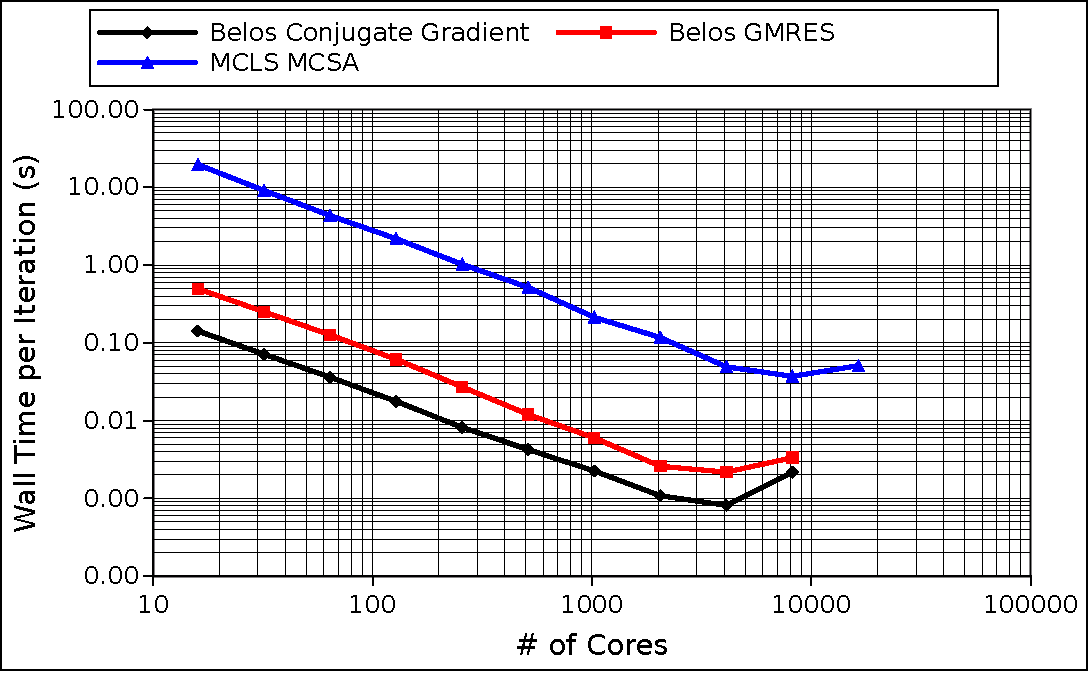
\includegraphics[width=3in]{titan_pure_strong_time.pdf}
  \end{center}
  \caption{Pure domain decomposition strong scaling wall time per
    iteration.}
  \label{fig:titan_pure_strong_time}
\end{figure}

\begin{figure}[h!]
  \begin{center}
    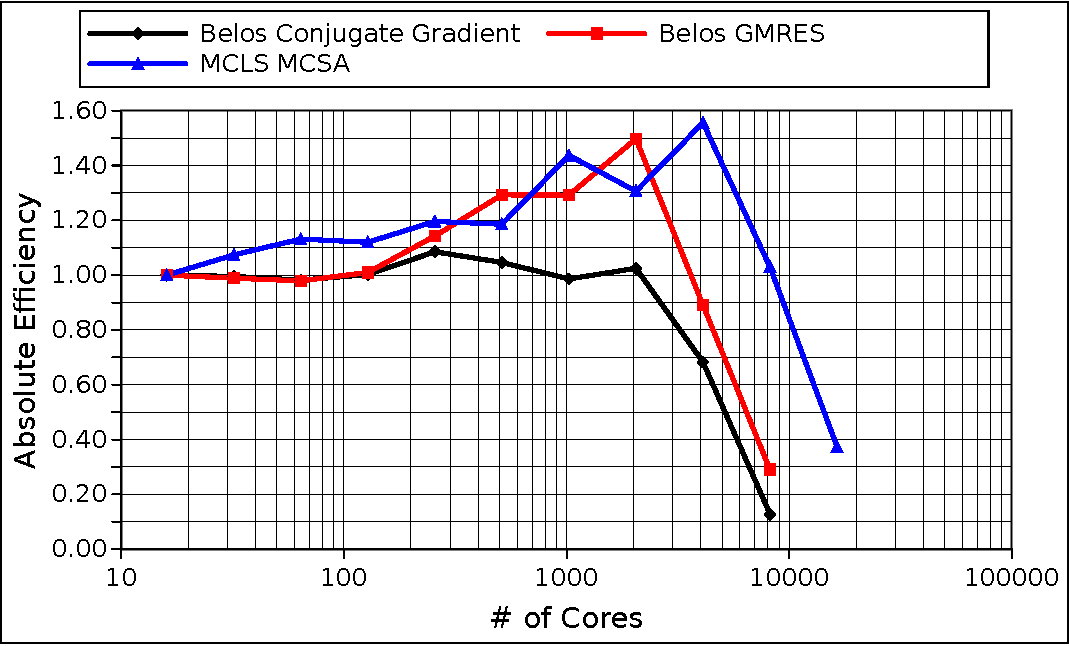
\includegraphics[width=3in]{titan_pure_strong.pdf}
  \end{center}
  \caption{Pure domain decomposition strong scaling absolute
    efficiency. \textit{Super-linear speed-up is from memory thrashing
      in the base case.}}
  \label{fig:titan_pure_strong}
\end{figure}

There are several key features of
Figure~\ref{fig:titan_pure_strong_time} and
Figure~\ref{fig:titan_pure_strong} worth noting. First, up to around
5,000 cores, all methods experience a super-linear improvement in
parallel efficiencies. For all methods, this increase is not a
function of the algorithmic efficiency as those computed using
Eq~(\ref{eq:algorithmic_efficiency}) remained at unity, meaning that
all computations converged in the same number of iterations relative
to the base case. Instead, what is happening here and was observed by
Brunner and Brantley in their work is that the large problem used to
scale to O(10,000) cores was large enough that memory thrashing was
occurring in the 16 core base case. As the number of cores in the
strong scaling study was increased and the local problem size
decreased, more of the local problem fit into the cache of the system,
thus causing improved serial performance and therefore enhanced run
times.

Beyond around 5,000 cores, the global problem size selected for this
strong scaling study causes the local problem size to shrink enough
that parallel communication costs begin to overtake arithmetic costs
on process. This takeover causes this effective strong scaling wall
that is observed in all methods. Using any more cores to solve this
particular global problem is not an efficient use of those parallel
resources. Furthermore, the fact that we see very similar trends in
efficiencies for all methods means that they are bound by the same
parallel performance limitations in a strong scaling environment. This
is important as we can expect the same qualitative scaling performance
from MCSA if arithmetic optimization has been performed to improve the
serial performance of the implementation. In addition, these results
are valuable in that they show MCSA, when properly parallelized, has
the ability to be competitive on leadership-class computing platforms
with conventional subspace methods with good strong scaling observed
in the pure domain decomposition case to O(10,000) cores.

Next, we consider the weak scaling performance of the algorithm. In
this case, we fix the local problem size at \sn{4}{4} DOFs and
increase the number of processors used in the
simulation. Figure~\ref{fig:titan_pure_weak_time} gives the wall time
per iteration and Figure~\ref{fig:titan_weak_absolute} gives the weak
scaling absolute efficiencies for this problem. Overall, weak scaling
performance of the parallel MCSA algorithm is excellent for the pure
domain decomposition case with absolute parallel efficiencies of over
80\% observed at over 32,000 cores.

\begin{figure}[p!]
  \begin{center}
    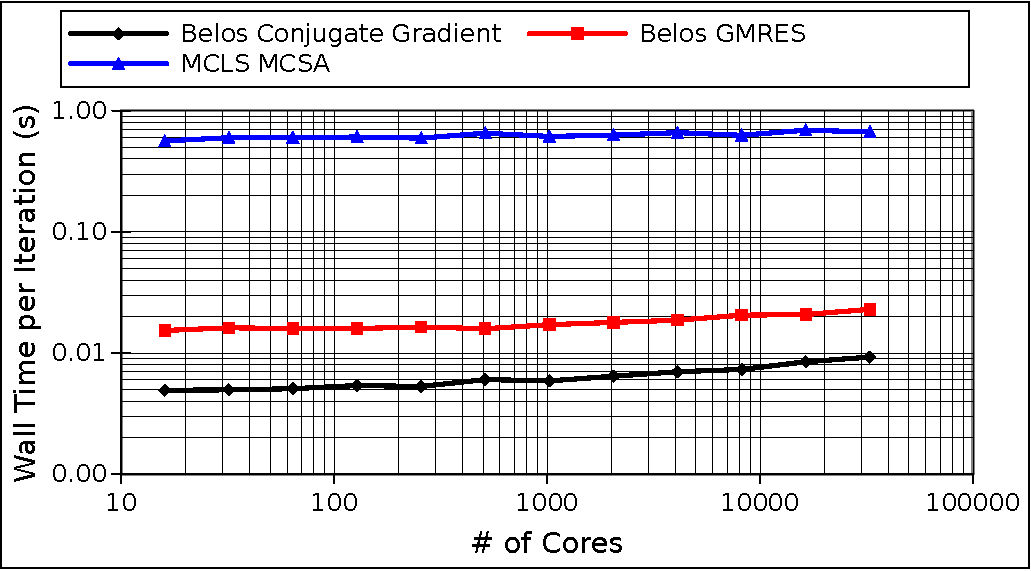
\includegraphics[width=3in]{titan_pure_weak_time.pdf}
  \end{center}
  \caption{Pure domain decomposition weak scaling wall time
      per iteration.}
  \label{fig:titan_pure_weak_time}
\end{figure}

\begin{figure}[h!]
  \begin{center}
    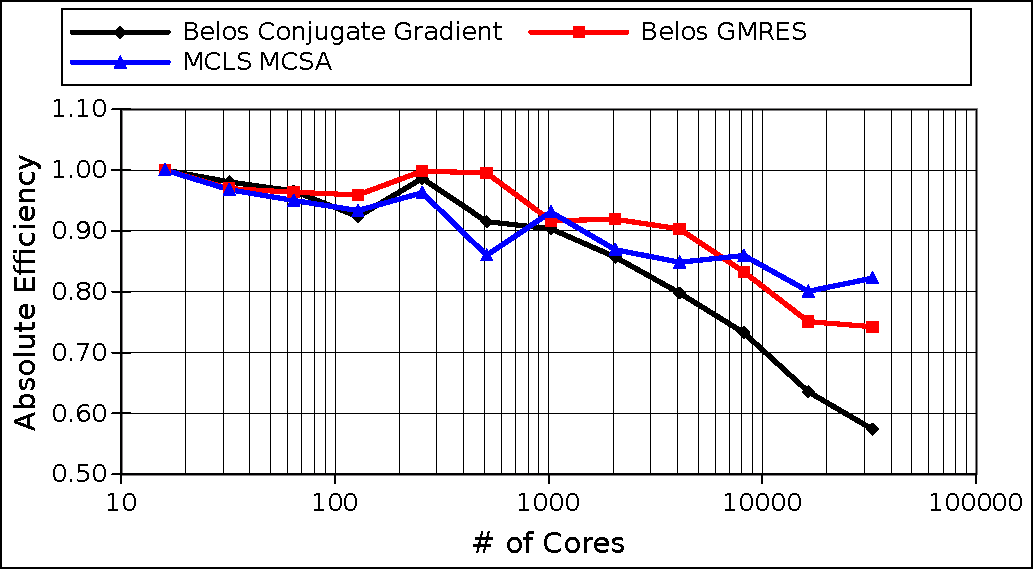
\includegraphics[width=3in]{titan_weak_absolute.pdf}
  \end{center}
  \caption{\textbf{Pure domain decomposition weak scaling absolute
      efficiency.} \textit{MCLS is an over order of magnitude slower
      arithmetically, causing the higher efficiency. GMRES executes
      more operations than conjugate gradient, also creating a higher
      efficiency.}}
  \label{fig:titan_weak_absolute}
\end{figure}

\subsection{Overlapping Domain Decomposition}
\label{subsec:overlapping_domain_decomp}
In the next set of scaling studies, we will explore how adding overlap
to the subdomains in the problem affects run times and parallel
performance as compared to the case with pure domain decomposition. To
do this, we utilize the set of analytic relations developed in
\cite{slattery_spectral_2013} to design these numerical
experiments. For the neutron diffusion problem used in these scaling
studies, the linear operator had a spectral radius of 0.787 and a
weight cutoff of \sn{1}{-2} was used with the Neumann-Ulam
solver. Using Eq~(\ref{eq:analytic_k}) gives an expected random walk
length of 19.22 transitions for any given history in the
problem. Using the mean-chord approximation given by
Eq~(\ref{eq:mean_chord_domain_leakage}), we then expect approximately
5.3\% of the histories born in a particular domain to leak out after
the first transport stage. By adding overlap, we aim to reduce this
fraction of communicated histories and therefore boost the parallel
performance of the algorithm.

To determine the amount of overlap to test for the scaling studies, we
use a variation of Eq~(\ref{eq:step_k_length}) to determine how many
discrete states a history will move on average from its birth site by
modifying it to only account for discrete movements:
\begin{equation}
  \sqrt{\bar{n^2_k}} = n_s \sqrt{k}\:,
  \label{eq:discrete_distance}
\end{equation}
where $\sqrt{\bar{n^2_k}}$ is now the root-mean-squared number of
discrete states a history will move from its birth site. For our
diffusion problem used in these scaling studies, we compute a value of
2.63 states per history for any of the dimensions of the system. This
means that we can expect to end up on average 2.63 states in both the
$i$ and $j$ dimensions away from the starting state. Therefore, we
will use the overlap generation algorithm outlined in
\S~\ref{subsec:msod_generation} such that we parametrically grow the
local domain using 1, 2, 3, and 5 levels to measure how scalability is
affected when this root-mean-squared number of states is
considered. For example, using 3 levels of overlap should keep over
50\% of the histories that would be communicated in the pure domain
decomposition case on-process as this is greater than the
root-mean-squared number of states we would expect a history to
travel.

For the performance metrics, we may use the same weak and strong
scaling efficiency metrics that we used for the pure domain
decomposition case. As we are comparing to the case without overlap
and are looking to boost performance relative to this case, for both
weak and strong scaling calculations we will use the 16-core case
without overlap as the reference computation for all efficiency
measures reported. The absolute efficiency results from the strong
scaling exercise are given in
Figure~\ref{fig:titan_strong_overlap}. Aside from the boosting of
efficiencies at 2,048 cores, little evidence of strong scaling
improvement is evident for all levels of overlap tested. 

To further explore any potential benefits of adding overlap into the
system, Figure~\ref{fig:titan_strong_overlap_diff} gives the
difference in the efficiencies between all overlap cases and the
reference case without overlap at each core count. At smaller numbers
of cores, there is no observed benefit to using overlap to improve
strong scaling. The improvements noted at 2,048 cores are also present
here and account for the best efficiency improvements for all core
counts tested. At 16,384 cores, using 2 levels of overlap did give a
6.4\% boost in efficiency while at 1,024 cores this same amount of
overlap actually reduced the efficiency. Beyond 2 levels of overlap,
efficiency levels begin to fall with 5 levels of overlap performing
the worst for all cases. From this, we don't expect adding any more
overlap will improve the scalability of the algorithm and the best
strong scaling performance was observed when the number of overlap
levels is approximately equal to the root-mean-squared number of
states we expect a history to move from its starting point as computed
by Eq~(\ref{eq:discrete_distance}).

\begin{figure}[h!]
  \begin{center}
    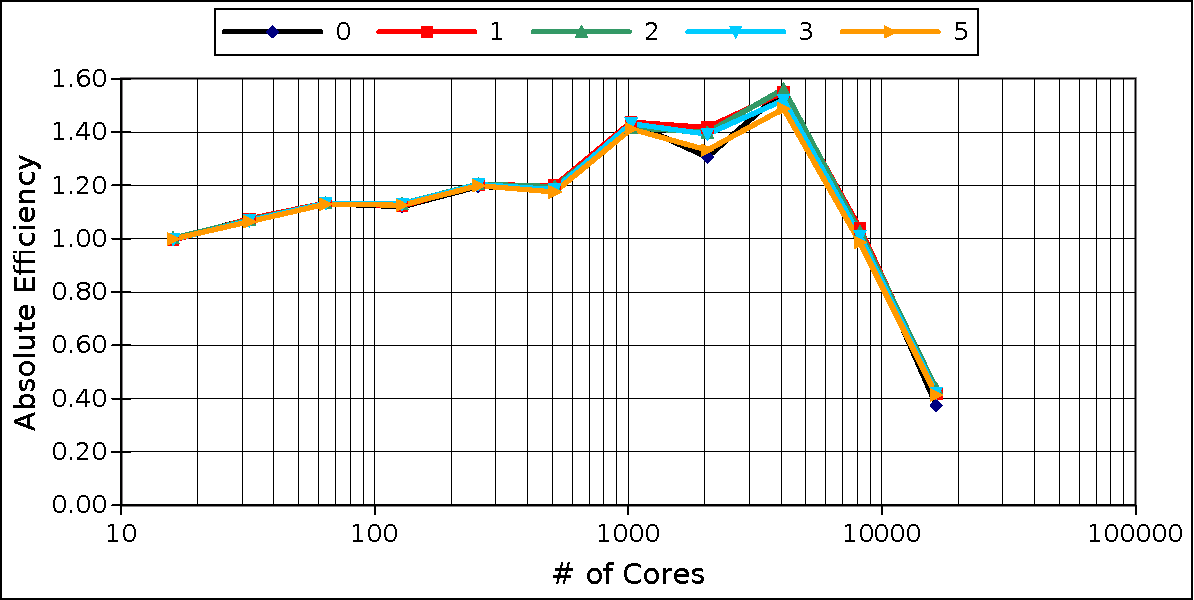
\includegraphics[width=3in]{titan_strong_overlap.pdf}
  \end{center}
  \caption{\textbf{Strong scaling absolute efficiency with varying
      levels of overlap.} \textit{Values of 0, 1, 2, 3, and 5 levels
      of overlap were used as the problem had a root-mean-squared
      number of states of 2.63 for each history.}}
  \label{fig:titan_strong_overlap}
\end{figure}

\begin{figure}[h!]
  \begin{center}
    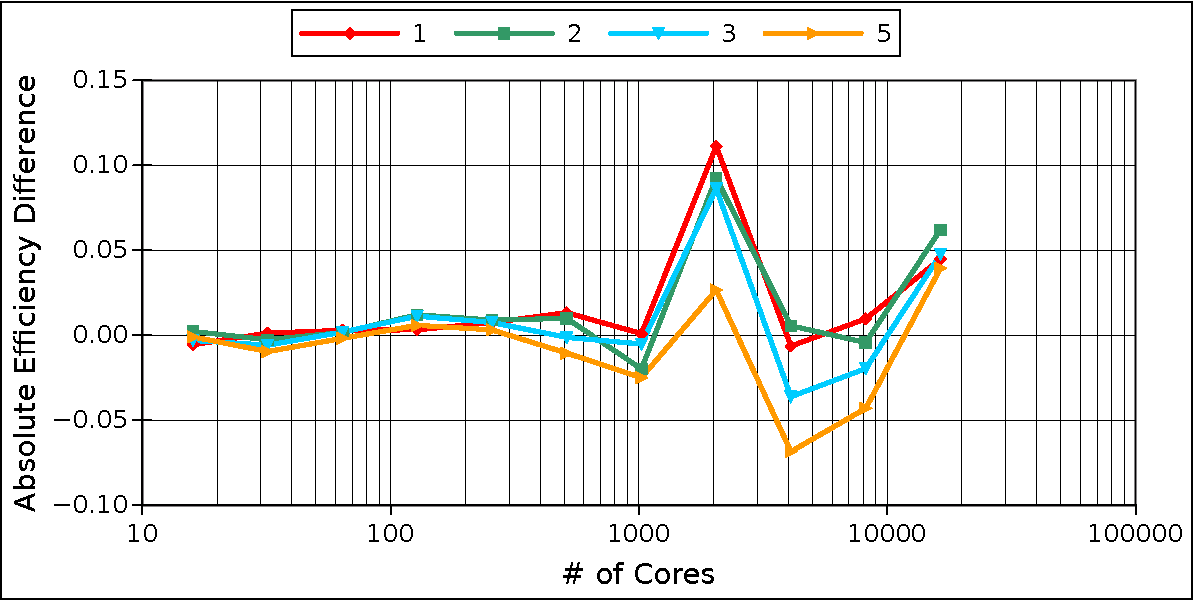
\includegraphics[width=3in]{titan_strong_overlap_diff.pdf}
  \end{center}
  \caption{\textbf{Strong scaling absolute efficiency difference with
      respect to the 0 overlap base case.} \textit{Values of 1, 2, 3,
      and 5 levels of overlap are compared here with the absolute
      difference of the absolute efficiencies presented.}}
  \label{fig:titan_strong_overlap_diff}
\end{figure}

For weak scaling, the same study as in the pure domain decomposition
case was performed again with 1, 2, 3, and 5 levels of overlap. The
absolute parallel efficiencies from these calculations are given in
Figure~\ref{fig:titan_weak_overlap} and the differences in
efficiencies from the calculations without overlap given in
Figure~\ref{fig:titan_weak_overlap_diff}. The results here are much
the same in that there is not a dramatic improvement in scalability
relative to the case without overlap. Opposite the strong scaling
calculation, overlap enhances weak scaling efficiencies at lower core
counts and degrades the efficiencies at higher core counts. In
addition, 1 level of overlap provided the best enhancement of
scalability when overlap was beneficial.

\begin{figure}[h!]
  \begin{center}
    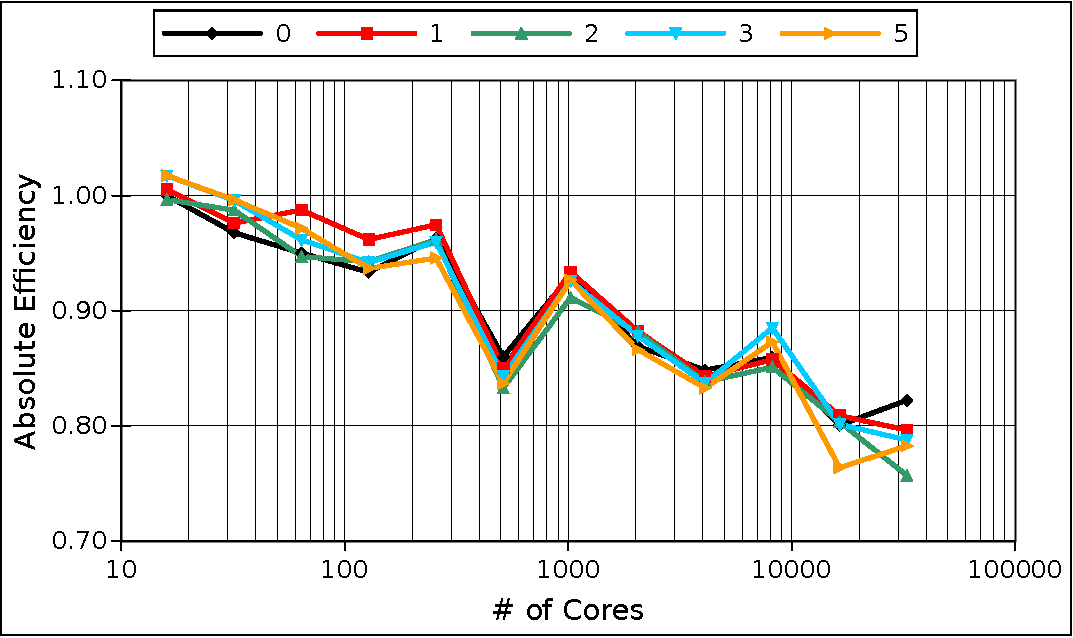
\includegraphics[width=3in]{titan_weak_overlap.pdf}
  \end{center}
  \caption{\textbf{Weak scaling absolute efficiency with varying
      levels of overlap.} \textit{Values of 0, 1, 2, 3, and 5 levels
      of overlap were used as the problem had a root-mean-squared
      number of states of 2.63 for each history.}}
  \label{fig:titan_weak_overlap}
\end{figure}

\begin{figure}[h!]
  \begin{center}
    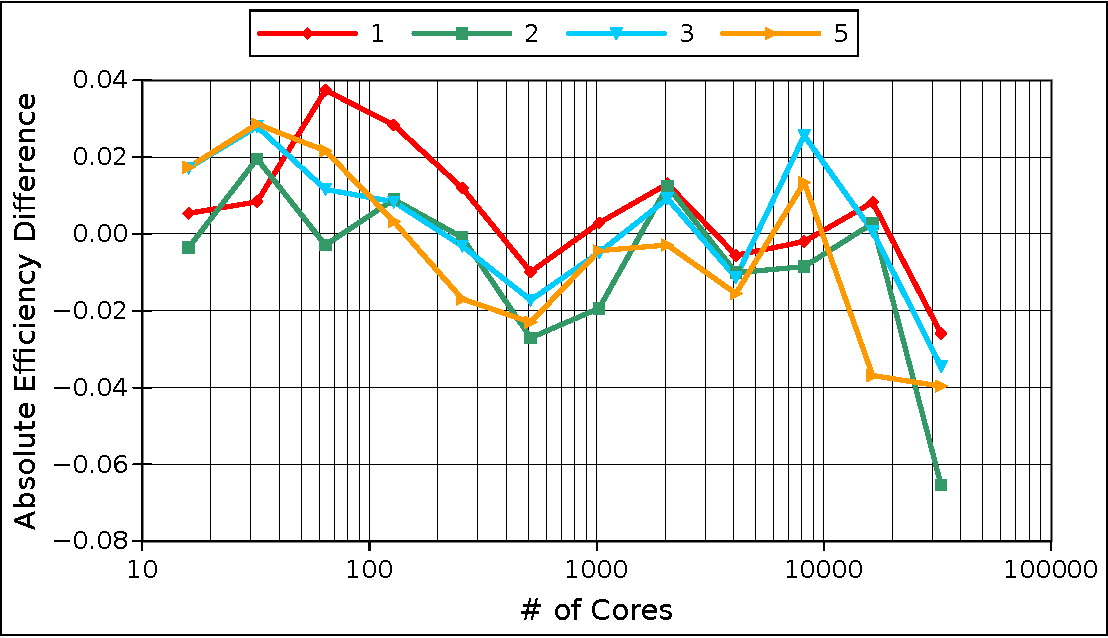
\includegraphics[width=3in]{titan_weak_overlap_diff.pdf}
  \end{center}
  \caption{\textbf{Weak scaling absolute efficiency difference with
      respect to the 0 overlap base case.} \textit{Values of 1, 2, 3,
      and 5 levels of overlap are compared here with the absolute
      difference of the absolute efficiencies presented.}}
  \label{fig:titan_weak_overlap_diff}
\end{figure}

For both the strong and weak scaling studies, the parallel performance
of the algorithm was either marginally improved or not improved at
all. We would always expect an improvement in performance for using
overlap to prevent the transport of histories from domain to domain
during execution of the Neumann-Ulam algorithm. The reduction in
transport means a reduction in parallel communication and therefore
should never degrade the performance of the algorithm. It is true that
doing so in fact enhances Monte Carlo performance. However, the
Neumann-Ulam algorithm is not representative of the entire MCSA
algorithm. When overlap is used, an overlapping tally vector is
constructed in parallel such that multiple cores may own multiple
states in the system. When this occurs, the tally data associated with
these shared states must be communicated after the Neumann-Ulam solve
as outlined in \S~\ref{subsec:msod_algorithm}. This reduction
operation then builds the full MCSA correction vector in the
decomposition of the solution vector. 

Therefore, by building overlap we are in fact reducing parallel
communication during the Neumann-Ulam solve but we are simply
deferring that communication until after Monte Carlo transport when
the overlapping tally vector must be reduced. When overlap becomes
large enough (i.e. larger than the root-mean-squared number of
discrete states a history will travel), then the savings in
communication during the Neumann-Ulam solve start to become smaller
than the communication created in the overlapping tally vector
reduction. We see this in both the strong and weak scaling cases at
larger levels of overlap. For the strong scaling case, we see better
performance improvement at higher core counts because the total number
of overlapping states on each core is smaller due to the local problem
size shrinking. For weak scaling, we see better performance
improvement at lower numbers of cores because although the local
overlap size is fixed, the global amount of overlap is growing with
core count and therefore reducing the performance of the tally
reduction operation.

\subsection{Multiple Set Domain Decomposition}
\label{subsec:ms_decomposition}
We next look to apply replication to the problem in the form of
multiple sets. As the previous analysis showed overlap to be of little
assistance in improving scalability, we only apply multiple sets to
the problem with pure domain decomposition within the sets for these
scaling studies. When adding sets, we must decide how many stochastic
histories to use to generate the correction vector in the MCSA
iteration. For this work we consider two choices; the split case and
the fully replicated case. As an example of these cases, consider a
single set problem where 20,000 histories are used in the Monte Carlo
solve. If we choose the split case, then solving the same problem with
2 sets would give 10,000 histories in each set and 4 sets would give
5,000 histories in each set. Splitting the histories in this way
provides the same global number of histories used to compute the
correction in the single set problem and we should therefore expect
the same iterative performance at a reduced time per iteration and
thus reduced time to solution. For the replicated history case, each
additional set in the problem will use just as many histories as the
single set case. Using 2 sets with fully replicated histories for our
example problem then has each set computing 20,000 histories with
40,000 global histories in the computation. For the 4 set case, the
number of global histories is increased to 80,000. By increasing the
global number of histories, the replicated cases should approximately
maintain time per iteration but should decrease the number of
iterations required to converge and subsequently reduce time to
solution.

\subsubsection{Strong Scaling with Multiple Sets}
\label{subsubsec:ms_strong}
For the strong scaling case, recall that the objective is to decrease
the time to solution for a given global problem size $N$ by increasing
$P$. Therefore, we may use Eqs~(\ref{eq:strong_scaling_absolute_ref}),
(\ref{eq:algorithmic_efficiency}), and
(\ref{eq:implementation_efficiency}) to compute the various strong
scaling efficiencies, but we must modify the reference computation in
each of these formulas to reflect our objective. For all efficiency
computations, the 16 core single set computation will be used as the
reference case. By adding more cores to the problem, either by
replicating with multiple sets, or decreasing the local problem size,
any computational resources added to the problem should aim to result
in speedup of this reference case. If this speedup for one technique
of adding cores is less than another, then that technique is deemed a
less efficient use of those computational resources.

For the multiple sets problem, the single set strong scaling study
from the pure domain decomposition base case was repeated for multiple
sets with both splitting of histories across sets and full replication
of histories across sets using both 2 and 4
sets. Figure~\ref{fig:titan_strong_ms_time} gives the actual wall
times for these computations. There are two important features to note
in the wall time data. First, splitting the histories among sets
instead of replicating them is faster due to the fact that cutting the
number of histories in half reduces the time of an iteration by a
factor that is nearly linear while increasing linearly the number of
histories through replication does not decrease the iterations
required to converge by a linear factor. Second, until the strong
scaling wall is hit starting at around 10,000 cores, the single set
case actually performs the fastest with only marginal improvement in
run times at higher numbers of cores with more sets. At these larger
numbers of cores, however, the improvements are so modest that one is
better off running the same problem using a single set at lower core
counts to conserve computational resources while maintaining a good
time to solution.

\begin{figure}[h!]
  \begin{center}
    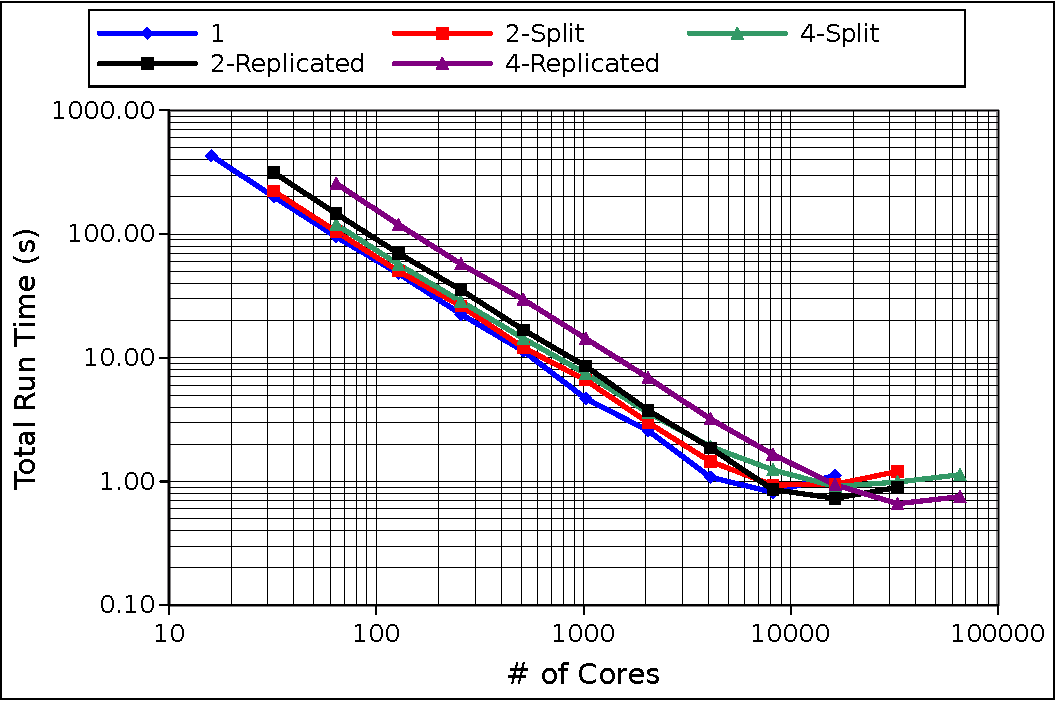
\includegraphics[width=3in]{titan_strong_ms_time.pdf}
  \end{center}
  \caption{\textbf{Wall time in seconds to solution for each case for
      the strong scaling study with multiple sets.} \textit{Until the
      strong scaling wall is reached at O(10,000) cores, the single
      set case performs the best. For the multiple set cases, it is
      faster to split histories among sets and maintain iterative
      performance rather than replicate histories to improve iterative
      performance.}}
  \label{fig:titan_strong_ms_time}
\end{figure}

From this timing data we compute the absolute efficiencies for strong
scaling as given in Figure~\ref{fig:titan_strong_ms_eff} using the
16-core single set calculation as the reference case. As observed in
the timing data, because the single set case had the fastest run times
up to the strong scaling wall it also has the best observed
efficiencies. For the 2 set case with history splitting, although the
time to perform an iteration was nearly cut in half, the extra
parallel overhead associated with reducing the tally across the blocks
to combine the set results increases run times and reduces
efficiencies. This reduction across blocks is even more obvious for
the 4 set case. Ultimately, all cases effectively hit the strong
scaling wall at the same time at around O(10,000) cores.

We expect this if we consider the fact that adding sets to the problem
is in itself effectively a form of strong scaling. For any given
problem of fixed size $N$, adding extra sets to the computation
decreases the global ratio of $N/P$ as $P$ will grow with the addition
of sets (although $N/P$ is constant within a set). For the split
history case, the splitting further exacerbates this situation by
further decreasing the amount of histories that will be computed in
the local domain, giving a larger ratio of communication to work in
the Monte Carlo solve. As with with single set results, we also
observe some efficiencies greater than unity for the multiple set
cases also due to improved cache utilization. 

Although not as dramatic as one might originally expect from
introducing replication, there are some modest gains in efficiencies
at high core counts by using multiple sets. Of interest here is where
the multiple set cases perform better than the single set case after
the single set case has hit the strong scaling wall. In
Figure~\ref{fig:titan_strong_ms_eff}, at 16,384 cores the single set
case operates at 38\% efficiency while at the same number of cores,
the 2 set case with history replication operates at 58\%
efficiency. Although the efficiencies here are still low, this is
reasonable improvement in the use of those computational resources,
gained by replicating the problem. Beyond 16,384 cores, there is not a
compelling reason to use more computational resources for this
problem.

\begin{figure}[h!]
  \begin{center}
    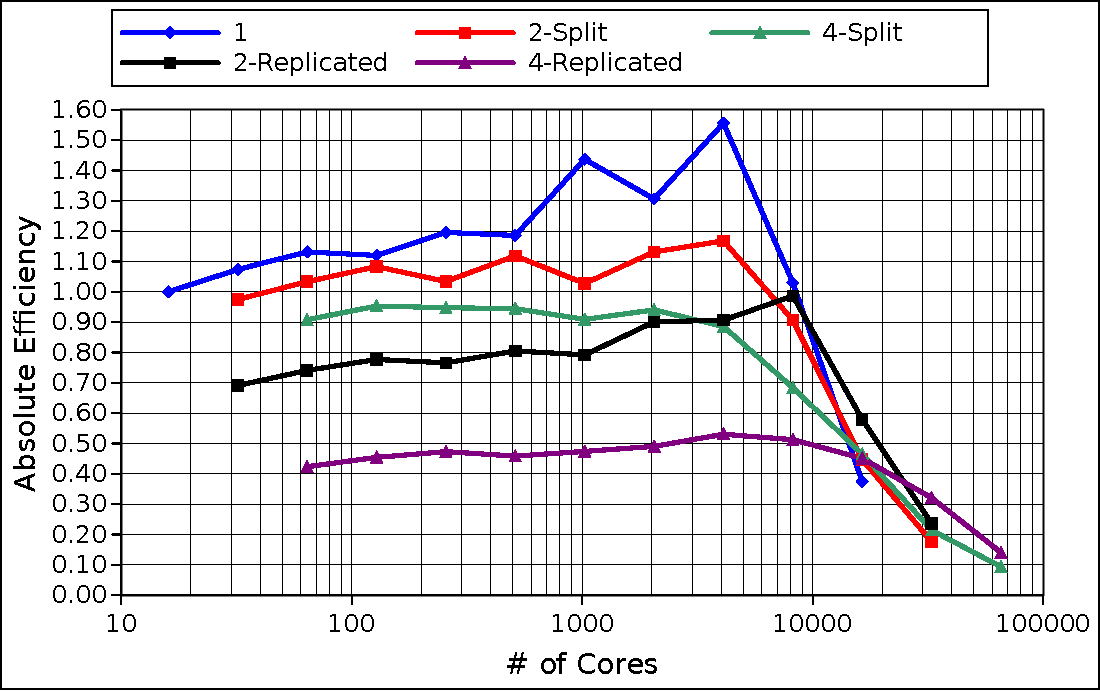
\includegraphics[width=3in]{titan_strong_ms_eff.pdf}
  \end{center}
  \caption{\textbf{Multiple set absolute parallel efficiency.}
    \textit{Computed relative to the 16-core 1-set base case. Using a
      single set is the best means by which to improve strong scaling
      up to the strong scaling wall. At higher core counts past where
      the single set case hits the strong scaling wall adding sets can
      provide some improvements in efficiencies.}}
  \label{fig:titan_strong_ms_eff}
\end{figure}

Also of interest here is the effect of splitting histories among sets
versus replicating them on the iterative performance of the
method. Table~\ref{tab:ms_strong_alg_eff} gives the iterations
required to converge and computed algorithmic efficiencies for each of
the cases presented in the strong scaling data. As expected, splitting
histories maintains a fixed global number of histories and therefore
maintained the number of iterations required to converge relative to
the single set base case. When histories were replicated, adding sets
decreased the number of iterations required to converge in a nonlinear
fashion. Therefore, increasing the number of histories per MCSA
iteration improves algorithmic efficiency. Using these algorithmic
efficiencies, the implementation efficiencies for the multiple set
cases were computed and are given in
Figure~\ref{fig:titan_strong_ms_impeff}. From these results, we see
that the replicated history cases are even less efficient than in the
absolute case with respect to the performance of a single
iteration. This is due to the fact that doubling the number of
histories does not halve the number of MCSA iterations required for
convergence as the acceleration is bound by the Central Limit
Theorem. As a result, the improved iterative performance from the
replicated cases comes at a higher cost in terms of time to solution
than the split cases.

\begin{table}[h!]
  \begin{center}
    \begin{tabular}{lcc}\hline\hline
      \multicolumn{1}{l}{Case}& 
      \multicolumn{1}{c}{Iterations}&
      \multicolumn{1}{c}{$\eta_{alg}$} \\\hline
      1 & 22 & 1.0 \\
      2-split & 22 & 1.0 \\
      2-replicated & 16 & 1.375 \\
      4-split & 22 & 1.0 \\
      4-replicated & 13 & 1.692 \\
      %%
      \hline\hline
    \end{tabular}
  \end{center}
  \caption{\textbf{Strong scaling algorithmic efficiency using
      multiple sets.} \textit{Replicating histories improves
      algorithmic efficiency by converging in fewer iterations.}}
  \label{tab:ms_strong_alg_eff}
\end{table}

\begin{figure}[h!]
  \begin{center}
    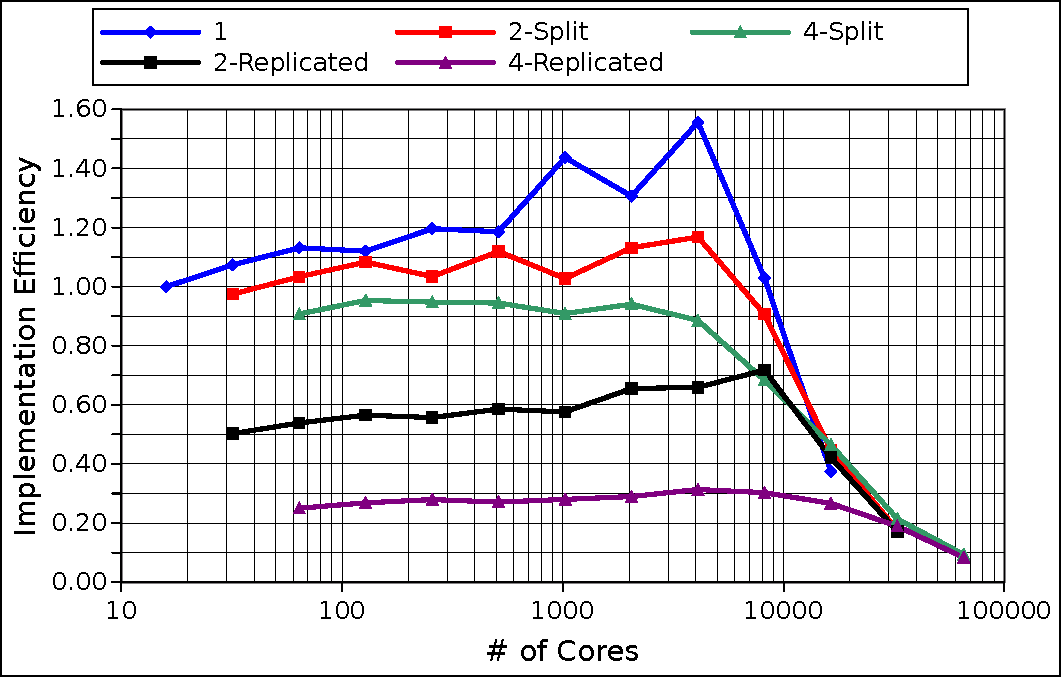
\includegraphics[width=3in]{titan_strong_ms_impeff.pdf}
  \end{center}
  \caption{\textbf{Multiple set strong scaling implementation
      efficiency.} \textit{Computed relative to the 16-core 1-set base
      case. Considering iterations required to converge, the
      performance of the split history cases is much better than the
      cases with history replication.}}
  \label{fig:titan_strong_ms_impeff}
\end{figure}

\subsubsection{Weak Scaling with Multiple Sets}
\label{subsubsec:ms_weak}
Next, we continue to a weak scaling study of the multiple sets
problem. In the same way as the strong scaling study, we will modify
the pure domain decomposition study to account for the additional
replication. For each calculation in the single set study, that
problem will be replicated either 2 or 4 times with both split and
replicated histories to assess the effects on scalability and
run time. Figure~\ref{fig:titan_weak_ms_time} gives the wall times from
the multiple sets weak scaling study. Of primary importance here is
the fact that adding sets to the problem with both split and
replicated histories actually decreases the time to solution. This was
not observed in the strong scaling case until much larger core counts
as the multiple set computations hit the strong scaling wall after the
single set computation.

This result is significant in that it shows a solution technique in
which the linear problem can actually be replicated and enhance time
to solution, something that cannot be achieved with conventional
methods. At larger core counts, however, this reduction in compute
time is not as large due to the fact that the tally reduction across
blocks requires more resources and those resources are clearly growing
with core count (most obviously in the 4 set case with split
histories). In addition, at 131,072 cores for the largest 4 set
computation, processors that share a block may be some physical
distance from one another in the machine, adding to latency and
decreasing performance.

\begin{figure}[h!]
  \begin{center}
    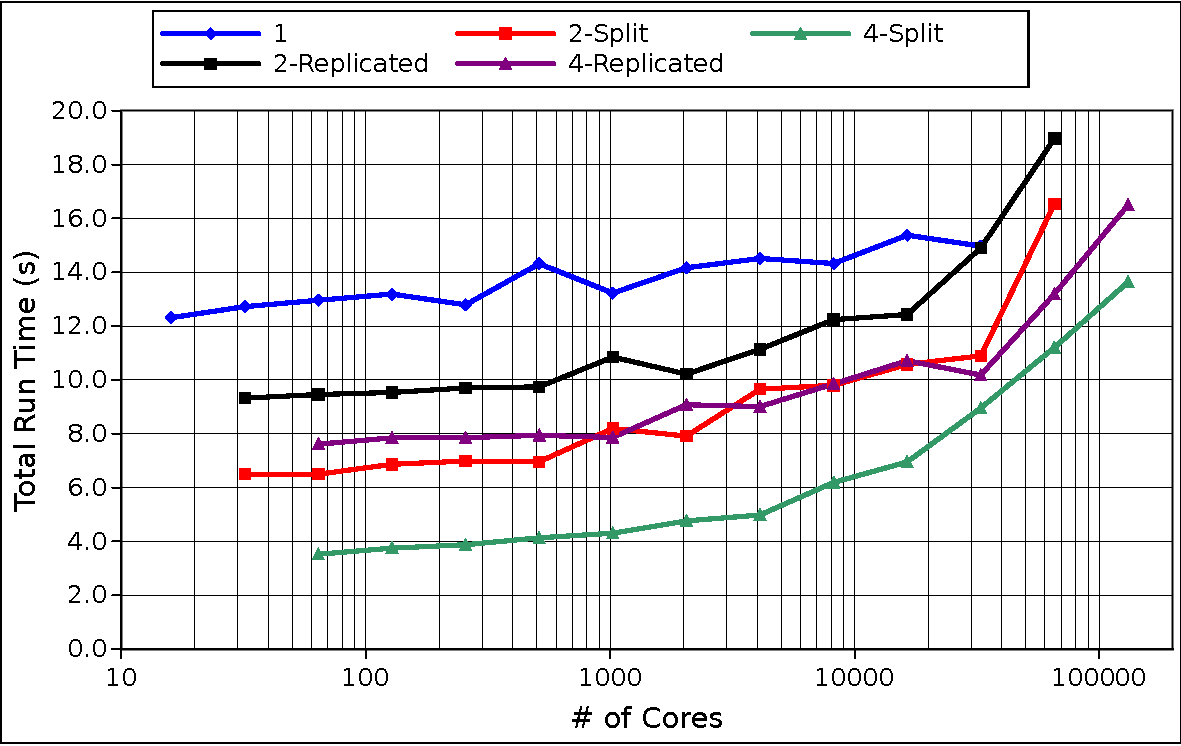
\includegraphics[width=3in]{titan_weak_ms_time.pdf}
  \end{center}
  \caption{\textbf{Wall time in seconds to solution for each case for
      the weak scaling study with multiple sets.}}
  \label{fig:titan_weak_ms_time}
\end{figure}

For a multiple set analysis of the weak scaling timing results, we
again have to consider that adding sets to the problem is actually a
form of strong scaling. Consider a single set problem ($S=1$) for a
given $P$ and $N$. When that problem is now solved using 2 sets we
have $S=2$, $N$, and $P=2P_s$ where $P_s$ is the number of processors in
a single set. For any number of sets we then have a global problem
size of $N$ while the number of processors is $SP_s$. Therefore,
$N/P$ is no longer fixed in the weak scaling study but rather
$N/(SP_s)$ is fixed. As a result, we modify the weak scaling absolute
efficiency relationship to account for this fact:
\begin{equation}
\eta_{weak}(M|N,P|Q,S) = \frac{T(M,Q)}{S \times T(N,P)}\:,
  \label{eq:ms_weak_efficiency}
\end{equation}
where now the absolute efficiency is a function of the number of sets
in the problem and again $M/Q = N/P$. As with the strong scaling
study, we will use the 16-core single set case as the reference
computation for efficiencies. Interestingly,
Eq~(\ref{eq:ms_weak_efficiency}) has a very similar form to the strong
scaling efficiency given by Eq~(\ref{eq:strong_scaling_absolute}),
representative of the strong scaling nature of adding additional
sets. For problems where adding sets improves time to solution, this
new weak scaling formulation accounts for how efficiently those extra
resources are incorporated into the problem.

Figure~\ref{fig:titan_weak_ms_eff} gives the results of the weak
scaling efficiency computations using the multiple set metric given by
Eq~(\ref{eq:ms_weak_efficiency}). Although we do reduce the time to
solution over the base cases for nearly all data points, the
observation here is that the reduction in time to solution is still
not large enough to efficiently use all resources. For example, for
the 2 set case to be a perfect use of resources with either split or
replicated histories, the run time of that calculation must be half of
that for the single set case. This was not the observation for the
run times in Figure~\ref{fig:titan_weak_ms_time} and therefore the
single set case is still the most efficient use of computational
resources in this scaling study.

\begin{figure}[h!]
  \begin{center}
    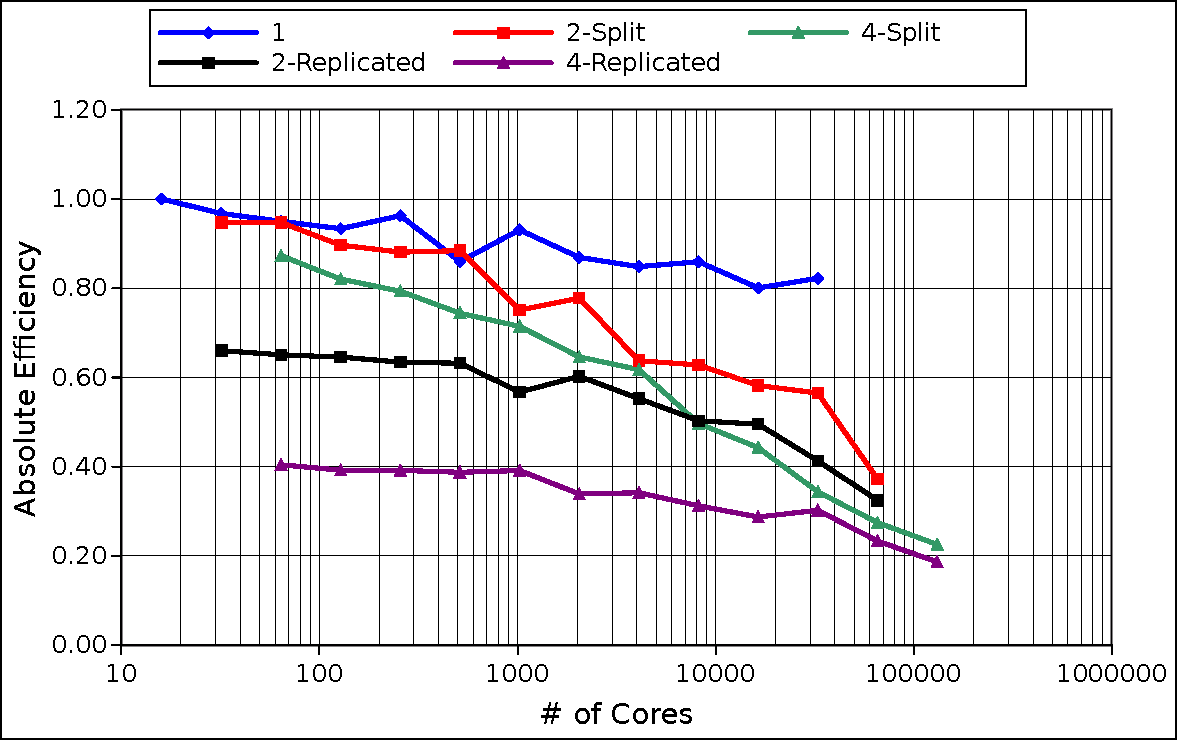
\includegraphics[width=3in]{titan_weak_ms_eff.pdf}
  \end{center}
  \caption{\textbf{Weak scaling absolute efficiency relative to
      16-core 1-set base case.}}
  \label{fig:titan_weak_ms_eff}
\end{figure}

As in the strong scaling case, splitting and replicating histories
across sets had effectively the same results for the weak scaling
study with the iterations to converge and computed algorithmic
efficiencies given by Table~\ref{tab:ms_weak_alg_eff}. The iterations
to converge these problems were not a function of problem size. Again,
when the implementation efficiencies are computed, we see in
Figure~\ref{fig:titan_weak_ms_impeff} that splitting histories among
sets is still a more efficient manner of introducing multiple sets
rather than replicating histories in an attempt to reduce the number
of iterations required to converge.  We also note that this is not a
true weak scaling study as indicated by
Eq~(\ref{eq:ms_weak_efficiency}) but rather an odd combination of both
weak and strong scaling. Regardless of this, although multiple sets
are not the most efficient use of resources in this analysis, they do
enhance the time to solution through replication and do so
significantly at core counts of O(1,000) and lower. In both the weak
and strong scaling cases, due to the additional computational and
communication overhead of adding sets to the system, one should never
expect to seriously boost parallel efficiencies for MCSA using this
technique except for certain instances past the strong scaling wall in
a purely strong scaling environment. In a weak scaling environment,
although no efficiency increase will be noted, one can expect an
enhancement of time to convergence by replicating.

\begin{table}[h!]
  \begin{center}
    \begin{tabular}{lcc}\hline\hline
      \multicolumn{1}{l}{Case}& 
      \multicolumn{1}{c}{Iterations}&
      \multicolumn{1}{c}{$\eta_{alg}$} \\\hline
      1 & 22 & 1.0 \\
      2-split & 22 & 1.0 \\
      2-replicated & 16 & 1.375 \\
      4-split & 22 & 1.0 \\
      4-replicated & 13 & 1.692 \\
      %%
      \hline\hline
    \end{tabular}
  \end{center}
  \caption{\textbf{Weak scaling algorithmic efficiency using multiple
      sets.} \textit{Replicating histories improves algorithmic
      efficiency by converging in fewer iterations.}}
  \label{tab:ms_weak_alg_eff}
\end{table}

\begin{figure}[h!]
  \begin{center}
    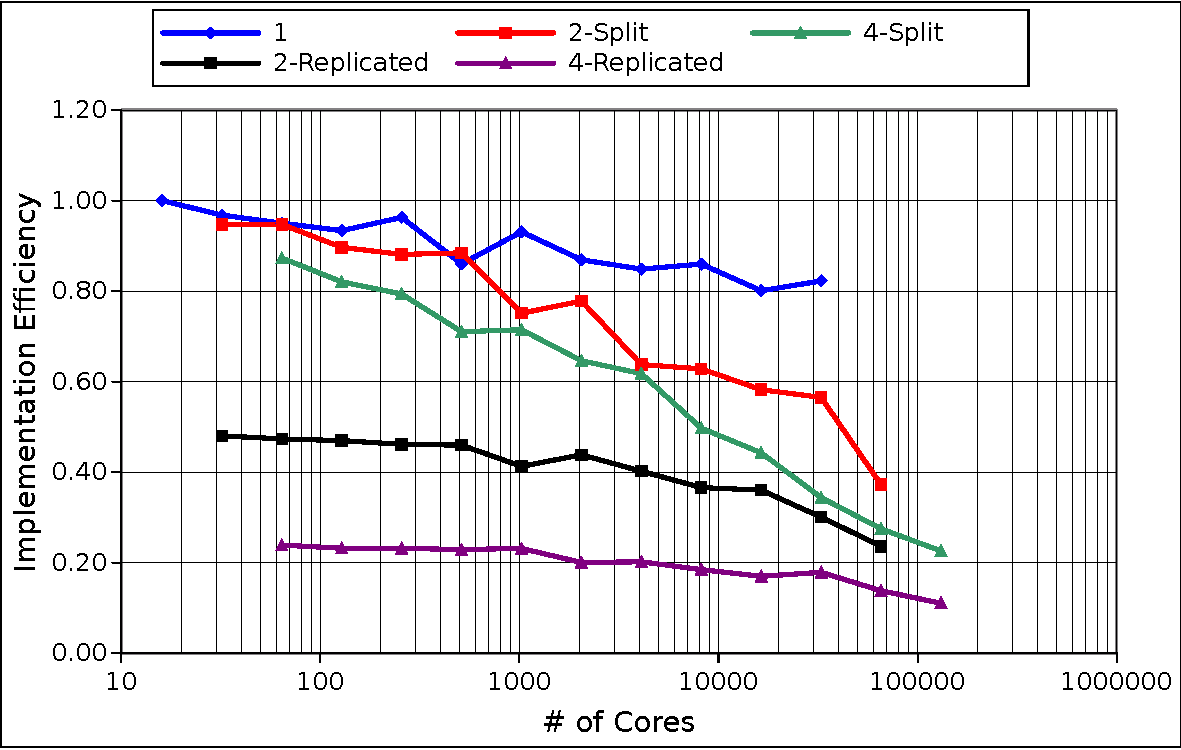
\includegraphics[width=3in]{titan_weak_ms_impeff.pdf}
  \end{center}
  \caption{\textbf{Implementation parallel efficiency relative to 16-core
      1-set base case.}}
  \label{fig:titan_weak_ms_impeff}
\end{figure}

%%%%%%%%%%%%%%%%%%%%%%%%%%%%%%%%%%%%%%%%%%%%%%%%%%%%%%%%%%%%%%%%%%%%%%%%%%%%%%%%
\section{Conclusions}

It was found the MCSA can indeed be effectively parallelized using the
multiple-set overlapping-domain decomposition algorithm borrowed from
the reactor physics community.  The new algorithm was tested in a wide
variety of parallel scaling studies on the Titan Cray XK7 machine at
the Oak Ridge Leadership Computing Facility. To test the algorithm at
high levels of concurrency, up to 65,356 cores were used in strong
scaling exercises and 131,072 cores used in weak scaling exercises
using a neutron diffusion problem.

Scaling studies showed that in the strong case overlap in small
quantities on the order of the mean-free-path of a stochastic history
in the simulation could boost parallel efficiencies by up to 10\% in
isolated cases. However, it was found that this additional overlap was
not effective in boosting weak scaling efficiencies. In general,
overlap was not very effective due to the fact that the parallel
communication saved during the Monte Carlo transport sequence is
simply deferred until after transport is complete when it manifests
itself as an overlapping parallel vector reduction operation. As
compared to transport calculations where this overlap procedure was
very effective, in the context of MCSA the Monte Carlo calculations
are significantly shorter with $O(10,000)$ histories used in this
work. These shorter calculations and more frequent overlapping tally
vector reductions create an overhead that is not observed in the
literature for transport calculations.

Applying multiple sets in the parallel algorithm was found to not
enhance the weak scaling of the problem as an additional parallel
overhead is introduced when the calculations from the set are combined
in superposition. For the strong scaling case, improvements were not
noted until after the strong scaling wall was hit. At this point,
multiple sets were observed to increase parallel efficiencies from
38\% to 58\% at 16,384 cores. Perhaps more important here is the fact
that although the parallel efficiency was reduced, multiple sets were
observed to actually improve the time to solution. Unlike a
traditional subspace method that we might apply to solve a neutron
transport problem, using MCSA means that we can actually make a
physical copy of the problem on the machine and can combine separate
Monte Carlo solutions for each copy through superposition. Time to
solution is then improved because fewer histories were run in each
copy and therefore each MCSA iteration is faster or more global
histories are computed and fewer MCSA iterations are required to
converge.

For future work, overall parallel scaling results indicated that the
implementation was of good quality in both the strong and weak scaling
cases. However, for the multiple set cases in the weak scaling
analysis, it was noted that there was a growing parallel overhead as a
function of core count. This was counter-intuitive in that the size of
the parallel group over which the set reductions were occurring was
fixed at all core counts and therefore we do not expect the addition
of such an operation to increase parallel run times. It did, however,
and therefore future research should explore why the implementation
for multiple sets generated parallel overhead that increased with core
count instead of remaining constant.


%%%%%%%%%%%%%%%%%%%%%%%%%%%%%%%%%%%%%%%%%%%%%%%%%%%%%%%%%%%%%%%%%%%%%%%%%%%%%%%%
\section*{Acknowledgments}

This work was performed under appointment to the Nuclear Regulatory
Commission Fellowship program at the University of Wisconsin - Madison
Department of Engineering Physics.

This research used resources of the Oak Ridge Leadership Computing
Facility at the Oak Ridge National Laboratory, which is supported by
the Office of Science of the U.S. Department of Energy under Contract
No. DE-AC05-00OR22725.

%%%%%%%%%%%%%%%%%%%%%%%%%%%%%%%%%%%%%%%%%%%%%%%%%%%%%%%%%%%%%%%%%%%%%%%%%%%%%%%%
\bibliographystyle{ans}
\bibliography{references}
\end{document}
